\colorbox{white!10!}{
    \begin{minipage}{0.2\textwidth}
       \begin{flushleft}
        \includegraphics[width = 0.6\textwidth]{Эмблема.png}
       \end{flushleft}
    \end{minipage}
    \begin{minipage}[t]{0.7 \textwidth}
        \begin{center}
            {\huge \textsc{Красноярская Летняя Школа. Сезон $7^2 - 2$}}
            \vspace{0.25cm}
            
            { \huge \textbf{ФМТ. Тур 5.1}}
        \end{center}
        \vspace{0.05cm}
    \end{minipage}
}

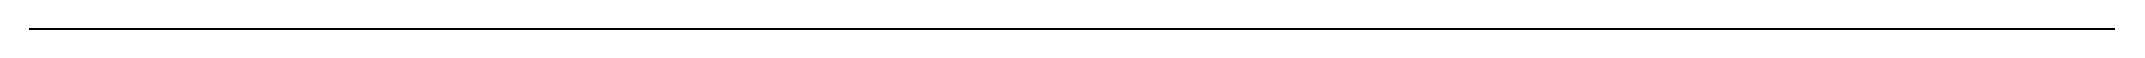
\begin{tikzpicture}
    \draw[thick] (-6.5,0)--(20,0);
\end{tikzpicture}
\begin{enumerate}

    \item Атлет бежит по круглому стадиону радиуса $r$, с постоянной по модулю скоростью $v$. Найти среднюю скорость перемещения спортсмена в момент времени $t = \tau$.
    
    \item Легкий стержень свободно висит, касаясь нижним концом поверхности воды, верхний конец шарнирно закреплен. Уровень воды начинает подниматься. Определить зависимость угла $\beta$ между стержнем и вертикалью от высоты $h$ уровня воды. Длина стержня равна $l$, а его плотность в $n$ раз меньше плотности воды.
    
\end{enumerate}